\section{Theorie}
\label{sec:Theorie}

\subsection{Interferenz von elektromagnetischen Wellen}
Im einfachsten Fall kann Licht als eine ebene elektromagnetische Welle dargestellt werden. Dabei hat der elektrische Feldanteil die Form
\begin{equation}
\vec{E}(x,t)=\vec{E}_.0\cdot \mathrm{e}^{i\left(kx -\omega t -\delta\right)}\label{eq:Welle},
\end{equation}
wobei $k$ die Wellenzahl und $\omega$ die Kreisfrequenz der Welle und $\delta$ eine Phasenverschiebung sind.
Aus den Maxwellgleichungen folgt, das mehrere solcher Wellen dem Superpositionsprinzip genügen und sich somit vektoriell addieren:
\[
\vec{E}=\vec{E}_.1+\vec{E}_.2+\text{...}
\]
Aufgrund der hohen Frequenzen der optischen Lichtwellen kann jedoch experimentell nur die Lichtintensität $I$, also der zeitliche Mittelwert der auf eine Fläche treffenden Leistung, bestimmt werden.
Es gilt:
\[
I=\frac{const}{t_.2-t_.1}\int_.{t_.1}^{t_.2}|\vec{E}(x,t)|^2\mathrm{d}t
\]
und somit bei Superposition von zwei Wellen
\begin{equation}
I_.{ges}=\frac{const}{t_.2-t_.1}\int_.{t_.1}^{t_.2}|\vec{E}_.1(x,t)+\vec{E}_.2(x,t)|^2\mathrm{d}t \text{.}
\end{equation}
Mit Gleichung folgt dann für die Intensität:
\begin{equation}
I_.{ges}=2\cdot const\cdot E^2_.0(1+\cos(\delta_.2-\delta_.1))
\end{equation}
Daraus lässt sich erkennen das, abhängig von der Phase der beiden Lichtwellen, die Intensität durch den Interferenzterm um bis zu $\pm 2\cdot const\cdot E^2_.0$ vom Mittelwert $2\cdot const\cdot E^2_.0$ abweichen.
Wenn gilt
\[
\delta_.2-\delta_.1=(2n+1)\pi,
\]
mit $n$ aus den natürlichen Zahlen, verschwindet die Intensität, selbst wenn die Einzelintensitäten von $0$ verschieden sind.
Dies gilt jedoch nur wenn für alle Phasenverschiebungen $\delta=const$ gilt. Wenn sie von der Zeit abhängen, führt eine zeitliche Mittelung über einen gegen die Periodendauer großen Zeitraum $t_.2-t_.1$ zum verschwinden des Interferenzterms. Das ist der Fall wenn das Licht inkoheränt ist, also wenn es nicht von derselben Lichtquelle ausgesandt wird.\newline
\begin{figure}
\centering
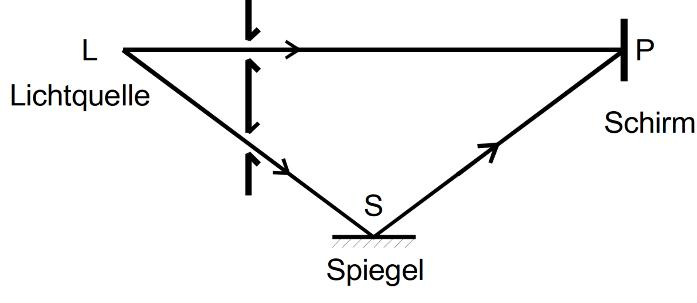
\includegraphics[scale=0.5]{content/images/kohaerenz.jpg}
\caption{Aufbau zur Erzeugung von kohärentem Licht\cite{V401}}
\label{fig:Kohärenz}
\end{figure}
Während das Licht eines Lasers immer kohärent ist, muss das einer gewöhnlichen Lichtquelle gemäß Abbildung \ref{fig:Kohärenz} durch Spiegelkonstruktionen oder Spalte aufgeteilt und umgelenkt werden, sodass es an einem Detektor durch die unterschiedlichen zurückgelegten Wegstrecken zu festen Phasenunterschieden kommt.
